% Appendix A

\chapter{Search heuristics for the Global algorithm} % Main appendix title

\label{AppendixB} % For referencing this appendix elsewhere, use \ref{AppendixA}

In section \ref{sec_LG_optimizations}, the efficient-oriented implementation of the combinatorial optimization problem that has to be solved by the Global algorithm is described. A way of exploring the space of combinations in decreasing $\mathbb{F}$ is needed to efficiently search for the optimal combination. In this appendix, the designed search heuristics to solve this problem are explained.

First of all, it must be assumed that the $S$ lists of $\Delta_i$ sub-solutions delivered by each satellite are ordered by decreasing $F$. This means that combination $\left(1 1 ... 1)\right)$ is the one which has the highest $\mathbb{F}$ value. However, this does not imply that this combination is the one that has a maximum $r(P)$ value.

Therefore, to explore the combinations space in decreasing $\mathbb{F}$, the combination $\left(1 1 ... 1)\right)$ has to be be the first one. The way to follow the exploration is explained below.

Let two key concepts for this explanation be defined (see also Fig. \ref{fig_succ}):
\begin{itemize}
\item A combination's \textbf{successor} is any other combination that is the selection of exactly the same sub-solutions as the first one except by one and only one satellite, for which it has selected the sub-solution immediately following the one that has selected the first combination in order of decreasing $\mathbb{F}$. For instance, the combination $\left(\mathbf{3} 3 2 4 0)\right)$ is the successor of $\left(2 3 \mathbf{2} 4 0)\right)$. Observe, however, that it is also successor of $\left(3 \mathbf{2} 2 4 0)\right)$.
\item In the same way, a combination's \textbf{predecessor} is any other combination that is the selection of exactly the same sub-solutions as the first one except by one and only one satellite, for which it has selected the sub-solution immediately preceding the one that has selected the first combination in order of decreasing F. $\left(2 3 \mathbf{2} 4 0)\right)$ and $\left(2 \mathbf{2} 2 5 0)\right)$ are predecessors of $\left(2 \mathbf{3} 2 \mathbf{5} 0)\right)$.
\end{itemize}

\begin{figure}[h!]
\centering
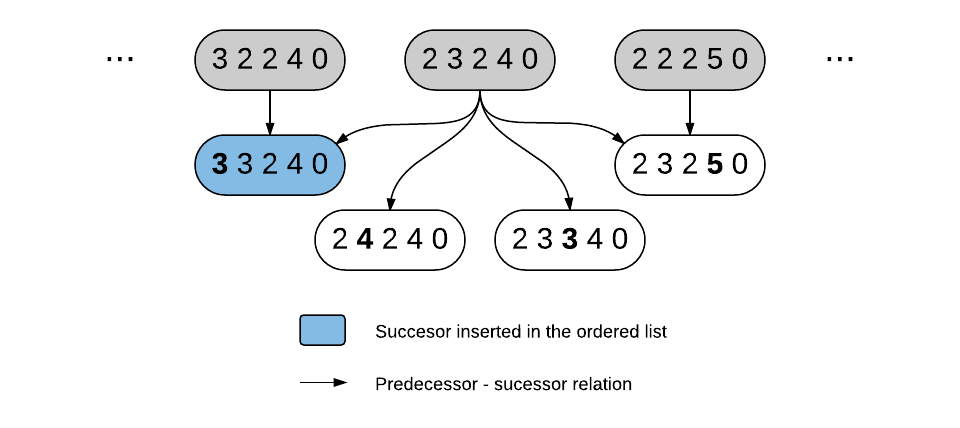
\includegraphics[scale=0.7]{Figures/succ.png} 
\caption{Predecessor and sucesors in the combinations space}
\label{fig_succ}
\end{figure}

Therefore, it can be proven that the exploration of the combinations space will be performed in decreasing $\mathbb{F}$ with the following procedure: for each combination being processed its successors are inserted in an ordered list and the first element in the list is selected as the following combination to be processed, starting from the combination $\left(1 1 ... 1)\right)$.

Noteworthy, a combination has more than one predecessor, so it would be inserted more than once in the ordered list, and hence it would be unnecessarily processed more than once. In order to insert the elements once and only once in the ordered list, each combination selects the successors to be inserted in the following way (see also the example of Fig. \ref{fig_succ}): from all the set of successors of a combination $c$ of the form $\left(1 1 ... c_k ... c_n)\right)$ where $c_k \in [2, \Delta_i]$ and $k \in [1,n]$, the inserted combinations subset is formed by all the successors of $c$ which differ from $c$ in any of the first $k$ components / satellite sub-solutions selections (e.g., the combination $(1 1 4 2 6)$ would insert $(2 1 4 2 6)$, $(1 2 4 2 6)$ and $(1 1 5 2 6)$).